\documentclass[11pt]{article}
\usepackage{anysize}
% ========================  PACKAGES =========================
\usepackage{amsmath, amssymb, amsthm, latexsym, color, textcomp, mathtools}
%\usepackage[ngerman, english]{babel}
%\usepackage[T1]{fontenc}
\usepackage[colorlinks=true,linkcolor=blue,citecolor=magenta,urlcolor=blue]{hyperref}
\usepackage{url}
\usepackage{tikz}
\usetikzlibrary{arrows,calc,shapes} 
\usetikzlibrary{external}
\tikzexternalize
% ============================================================

\newcommand{\size}{\operatorname{size}} 


\begin{document}
\title{Some small fat rational polytopes}
\author{Moritz Firsching}
\maketitle
\vspace{-3.9cm}
\begin{figure}[!ht]\centering
\tikzsetnextfilename{plot} 
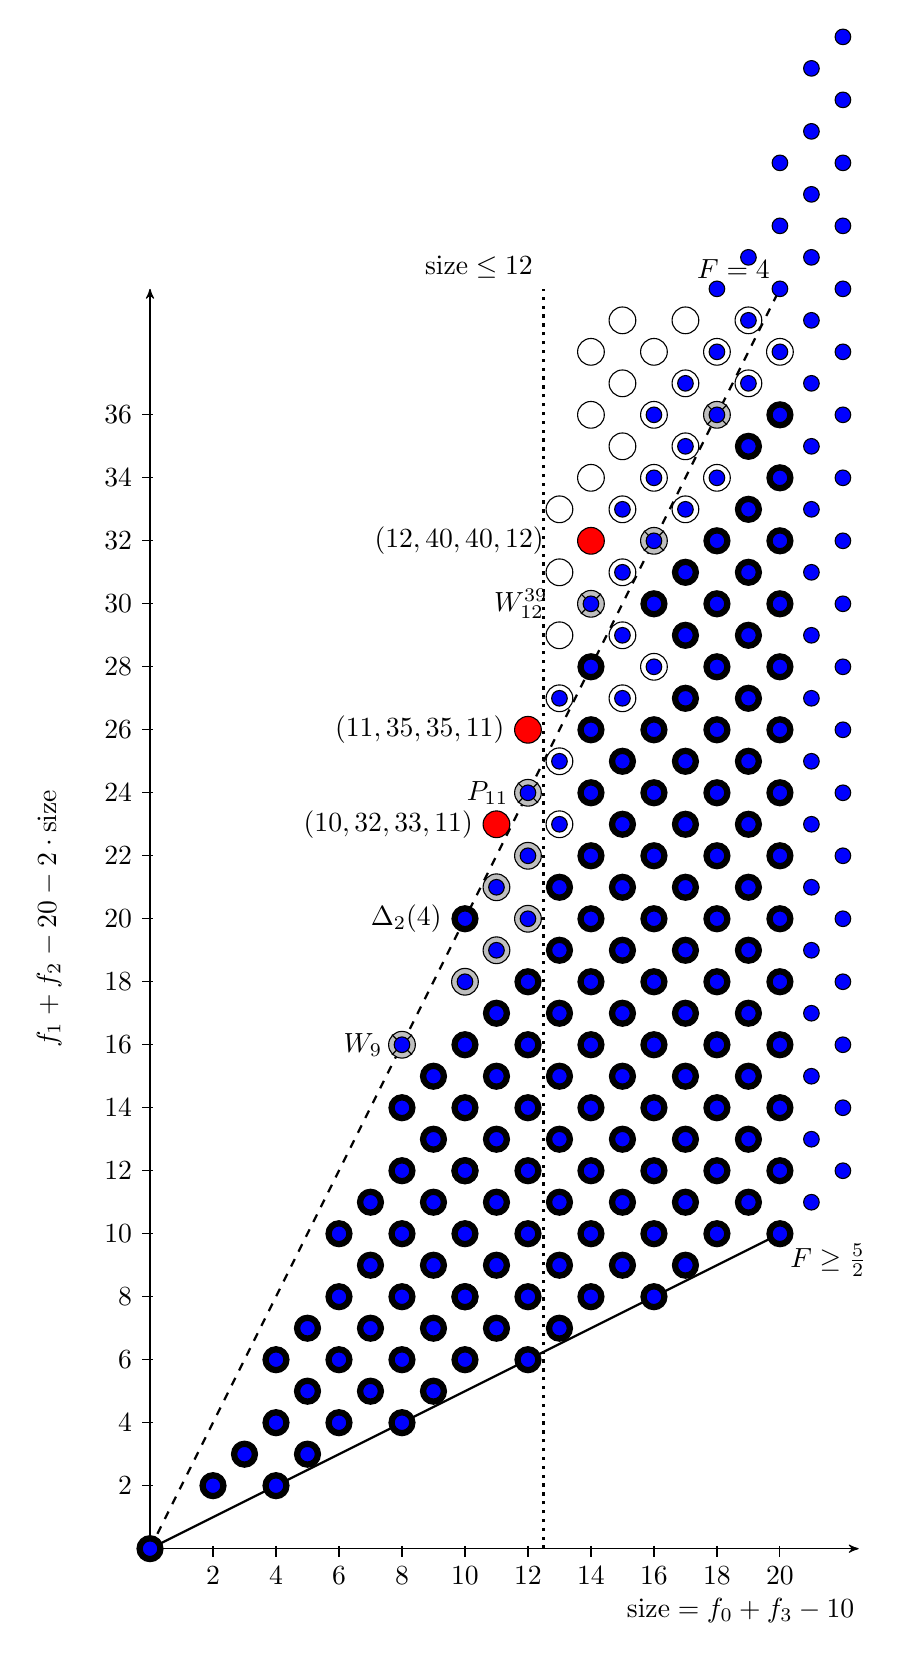
\begin{tikzpicture}[scale=1,>=stealth']
	%Achsen
    \draw[->] (0,0) -- coordinate (x axis mid) (9,0);
    \draw[->] (0,0) -- coordinate (y axis mid)(0,16);
    \foreach \t in {2,4,6,8,10,12,14,16,18,20}{
    	\edef\x{\t}
        \draw [](4*\x mm,1pt) -- (4*\x mm,-3pt)
            node[anchor=north] {$\x$};
    }
    \foreach \t in {2,4,6,8,10,12,14,16,18,20,22,24,26,28,30,32,34,36}{
    	\edef\y{\t}
        \draw (1pt,4*\y mm) -- (-3pt,4*\y mm) node[anchor=east] {$\y$};
    }
    \node[below=.5cm, name=X] at (x axis mid) {\hspace{60mm}$\size=f_0+f_3-10$};
    \node[rotate=90,above=1cm] at (y axis mid) {$f_1+f_2-20-2\cdot\size$};

    %Linien
    \draw[thick] (0,0)--(8,4) node[below right] {$F\geq\frac{5}{2}$};
    \draw[thick,dashed] (0,0)--(8,16) node[above left] {$F=4$};
    \draw[very thick,dotted] (0.4*12.5,0)--(0.4*12.5,16) node[above left] {$\size\leq 12$};

    % schwarze Punkte
    \foreach \x/\y/\beschriftung in {0/0/{}, 2/2/{}, 3/3/{}, 4/2/{}, 4/4/{}, 4/6/{},
    								 5/3/{}, 5/5/{}, 5/7/{}, 6/4/{}, 6/6/{}, 6/8/{}, 6/10/{},
    								 7/5/{}, 7/7/{}, 7/9/{}, 7/11/{}, 8/4/{}, 8/6/{}, 8/8/{},8/10/{},8/12/{},8/14/{},
    								 9/5/{}, 9/7/{}, 9/9/{}, 9/11/{}, 9/13/{}, 9/15/{},
    								 10/6/{}, 10/8/{}, 10/8/{}, 10/10/{}, 10/12/{}, 10/12/{}, 10/14/{}, 10/16/{},
    								 10/20/{$\Delta_2(4)$},
    								 11/7/{}, 11/9/{}, 11/11/{}, 11/13/{}, 11/15/{}, 11/17/{},
    								 12/6/{}, 12/8/{}, 12/10/{}, 12/12/{}, 12/14/{}, 12/16/{}, 12/18/{},
    								 13/7/{}, 13/9/{}, 13/11/{}, 13/13/{}, 13/15/{}, 13/17/{}, 13/19/{}, 13/21/{},
    								 14/8/{}, 14/10/{}, 14/12/{}, 14/14/{}, 14/16/{}, 14/18/{}, 14/20/{}, 14/22/{},
    								 14/24/{}, 14/26/{}, 14/28/{},
    								 15/9/{},15/11/{},15/13/{},15/15/{},15/17/{},15/19/{},15/21/{},15/23/{},15/25/{},
    								 16/8/{}, 16/10/{}, 16/12/{}, 16/14/{}, 16/16/{}, 16/18/{}, 16/20/{}, 16/22/{},
    								 16/24/{}, 16/26/{}, 16/30/{},
    								 17/9/{}, 17/11/{}, 17/13/{}, 17/15/{}, 17/17/{}, 17/19/{}, 17/21/{}, 17/23/{},
    								 17/25/{}, 17/27/{}, 17/29/{}, 17/31/{},
    								 18/10/{}, 18/12/{}, 18/14/{}, 18/16/{}, 18/18/{}, 18/20/{}, 18/22/{}, 18/24/{},
    								 18/26/{}, 18/28/{}, 18/30/{}, 18/32/{},
    								 19/11/{}, 19/13/{}, 19/15/{}, 19/17/{}, 19/19/{}, 19/21/{}, 19/23/{}, 19/25/{},
    								 19/27/{}, 19/29/{}, 19/31/{}, 19/33/{}, 19/35/{},
    								 20/10/{}, 20/12/{}, 20/14/{}, 20/16/{}, 20/18/{}, 20/20/{}, 20/22/{}, 20/24/{},
    								 20/26/{}, 20/28/{}, 20/30/{}, 20/32/{}, 20/34/{}, 20/36/{}
    								}{
        \draw (0.4*\x,0.4*\y)node[circle,radius=0.100, draw, fill=black, label={left:\beschriftung}] {};
    }	

    %rote Punkte
    \foreach \x/\y/\beschriftung in {11/23/{$(10,32,33,11)$}, 
										%12/24/{$(10,33,35,12)$}, 
										12/26/{$(11,35,35,11)$},
									 	14/32/{$(12,40,40,12)$\hspace{3mm}}
    								}{
        \draw (0.4*\x,0.4*\y)node[circle, inner sep=1.2mm, draw=black, fill=red, label={left:\beschriftung}] {};
    }
    %graue Punkte
    \foreach \x/\y/\beschriftung in {10/18/{}, 11/19/{}, 11/21/{}, 12/20/{}, 12/22/{}
    								}{
        \draw (0.4*\x,0.4*\y)node[circle, inner sep=1.2mm, draw=black, fill=black!25, label={left:\beschriftung}] {};
    }

    \foreach \x/\y/\beschriftung in {8/16/{$W_9$}, 12/24/{$P_{11}$}, 16/32/{}, 18/36/{},
									14/30/{$W_{12}^{39}$\hspace*{3mm}}
    								}{
        \draw (0.4*\x,0.4*\y)node[circle, inner sep=1.2mm, draw, fill=black!25] {};
        \draw (0.4*\x,0.4*\y)node[circle, inner sep=1.2mm, cross out, draw, label={left:\beschriftung}] {};
    }
    %leere Kreise
    \foreach \x/\y/\beschriftung in {13/23/{}, 13/25/{}, 13/27/{}, 13/29/{}, 13/31/{}, 13/33/{}, 14/34/{},
    								 14/36/{}, 14/38/{}, 15/27/{}, 15/29/{}, 15/31/{}, 15/33/{},
    								 15/35/{}, 15/37/{}, 15/39/{}, 16/28/{}, 16/34/{}, 16/36/{},
    								 16/38/{}, 17/33/{}, 17/35/{}, 17/37/{}, 17/39/{}, 18/34/{}, 18/38/{},
    								 19/37/{}, 19/39/{}, 20/38/{}
    								}{
        \draw (0.4*\x,0.4*\y)node[circle, inner sep=1.2mm, draw=black, fill=white, label={left:\beschriftung}] {};
    }  
    % blaue Punkte   
	\foreach \x/\y/\beschriftung in {15/21/{}, 16/20/{}, 18/26/{}, 20/20/{}, 22/26/{}, 10/6/{}, 14/22/{}, 20/38/{}, 17/21/{}, 21/37/{}, 2/2/{}, 22/44/{}, 13/17/{}, 18/10/{}, 15/23/{}, 16/22/{}, 19/39/{}, 4/2/{}, 18/28/{}, 20/22/{}, 5/3/{}, 12/18/{}, 22/28/{}, 19/11/{}, 14/24/{}, 20/40/{}, 17/23/{}, 21/39/{}, 11/7/{}, 22/46/{}, 6/4/{}, 10/20/{}, 13/19/{}, 18/12/{}, 15/25/{}, 16/24/{}, 19/41/{}, 18/30/{}, 22/12/{}, 14/8/{}, 20/24/{}, 5/5/{}, 8/4/{}, 12/20/{}, 0/0/{}, 22/30/{}, 11/9/{}, 14/26/{}, 20/42/{}, 21/41/{}, 15/9/{}, 6/6/{}, 16/8/{}, 7/5/{}, 13/21/{}, 18/14/{}, 16/26/{}, 22/14/{}, 14/10/{}, 20/26/{}, 17/9/{}, 21/25/{}, 12/22/{}, 9/5/{}, 5/7/{}, 22/32/{}, 14/28/{}, 20/44/{}, 21/43/{}, 15/11/{}, 16/10/{}, 7/7/{}, 13/23/{}, 19/27/{}, 18/16/{}, 16/28/{}, 20/10/{}, 12/6/{}, 3/3/{}, 22/16/{}, 14/12/{}, 17/11/{}, 20/28/{}, 21/27/{}, 9/7/{}, 12/24/{}, 14/30/{}, 21/45/{}, 10/8/{}, 13/7/{}, 15/13/{}, 16/12/{}, 19/29/{}, 7/9/{}, 18/18/{}, 16/30/{}, 20/12/{}, 21/11/{}, 12/8/{}, 22/18/{}, 4/4/{}, 14/14/{}, 20/30/{}, 21/29/{}, 9/9/{}, 21/47/{}, 10/10/{}, 13/9/{}, 19/13/{}, 17/25/{}, 16/14/{}, 7/11/{}, 19/31/{}, 22/48/{}, 20/14/{}, 21/13/{}, 12/10/{}, 15/27/{}, 22/20/{}, 4/6/{}, 14/16/{}, 20/32/{}, 18/32/{}, 21/31/{}, 8/6/{}, 19/15/{}, 10/12/{}, 13/11/{}, 11/11/{}, 17/27/{}, 19/33/{}, 16/16/{}, 6/8/{}, 20/16/{}, 21/15/{}, 12/12/{}, 15/29/{}, 14/18/{}, 18/34/{}, 21/33/{}, 8/8/{}, 22/34/{}, 19/17/{}, 10/14/{}, 11/13/{}, 17/29/{}, 19/35/{}, 6/10/{}, 13/25/{}, 20/18/{}, 21/17/{}, 12/14/{}, 15/31/{}, 18/36/{}, 21/35/{}, 17/13/{}, 8/10/{}, 19/19/{}, 22/36/{}, 10/16/{}, 11/15/{}, 17/31/{}, 19/37/{}, 15/15/{}, 13/27/{}, 18/20/{}, 21/19/{}, 12/16/{}, 15/33/{}, 16/32/{}, 18/38/{}, 17/15/{}, 8/12/{}, 9/11/{}, 22/38/{}, 19/21/{}, 10/18/{}, 11/17/{}, 17/33/{}, 15/17/{}, 18/22/{}, 21/21/{}, 16/34/{}, 18/40/{}, 22/22/{}, 20/34/{}, 17/17/{}, 8/14/{}, 9/13/{}, 22/40/{}, 19/23/{}, 11/19/{}, 17/35/{}, 13/13/{}, 15/19/{}, 16/18/{}, 18/24/{}, 21/23/{}, 16/36/{}, 22/24/{}, 14/20/{}, 20/36/{}, 8/16/{}, 17/19/{}, 9/15/{}, 22/42/{}, 19/25/{}, 11/21/{}, 17/37/{}, 13/15/{}}{
	        \draw (0.4*\x,0.4*\y)node[circle,inner sep=.7mm,radius=0.0050, draw, fill=blue, label={left:\beschriftung}] {};
    }
\end{tikzpicture}
\caption{Blue dots signify the existence at a rational polytope with a corresponding $f$-vector, compare \cite[Figure 3]{BZ18}}
\end{figure}
\clearpage

In order to realize missing polytopes from \cite[Figure 3]{BZ18}, we provide a short program written in Sage \cite{SageMath} to randomly generate rational polytopes and then optimize for certain properties. During the optimization we systematically remove vertices and facets and greedily take the resulting polytope if it improves the desired property. Instead of removing vertices and facets one could instead use other modifications of the polytopes, but this approach seems to work reasonably well for the purpose of optimizing the fatness paramater at hand. At \cite{F21} we give the code and a list of rational polytopes.  We look at a pair $(\size, f_1 + f_2 - 20 - 2\cdot \size)$, for which we haven't found a rational realization yet and, as a property, minimize the euclidean distance to that pair. We restrict the search to $\size \leq 22$ and can recover realizations for all known pairs $(\size, f_1 + f_2 - 20 - 2\cdot \size)$ and find a few previously unknown pairs. 
\bibliographystyle{alpha}
\bibliography{ref}

\end{document}
